\documentclass[onlytextwidth, aspectratio=169]{beamer}
\documentclass[onlytextwidth, aspectratio=169]{beamer}
\usepackage[utf8]{inputenc}
\usepackage{microtype}
\usepackage{amsmath}
\usepackage{amssymb}
\usepackage[nomessages]{fp} %\FPeval{\var-name}{2*sin(pi/6)}
\usepackage{siunitx} %units in math. eg 20\milli\meter
\usepackage{yhmath} % for arcs, overparenth command
\usepackage{tikz} %graphics
\usetikzlibrary{quotes, angles, arrows, arrows.meta}
%\usepackage{graphicx} already loaded by beamer class
%consider setting \graphicspath{{images/}}
%\parskip ?? to avoid paragraph indent
\usepackage{multicol} %may not need this package, just columns environment
\usepackage{venndiagram}

\subtitle[BECA]{Bronx Early College Academy}
\author[Huson]{Christopher J. Huson PhD}

\setbeamertemplate{headline}{\vskip2mm 
  \, BECA / \insertshortauthor \, / \inserttitle
  \hfill 
  \insertsection
  }

%Tick mark commands
\newcommand\ticks{}
  \def\ticks{{Bar[scale=2]}-{Bar[scale=2]}}
\newcommand\paraticks{}
  \def\paraticks{{Straight Barb[reversed, scale=2]}-{Straight Barb[scale=2]}}

\title{Geometry Unit 10: Trigonometry}
\date{17 April 2023 - 5 May 2023}

\begin{document}
\frame{\titlepage}
\section[Outline]{}
\frame{\tableofcontents}

\section{10.1 Slope and the tangent function \hfill 17 April \,}
\begin{frame}{Learning Target: I can convert angle measures to slopes using the tangent function.}
  {HSG.SRT.C.8 Use trigonometric ratios and the Pythagorean Theorem to solve problems \hfill \alert{10.1 Monday 17 April}}
  \begin{columns}
    \column{0.5\textwidth}
    Do Now: Given right $\triangle$, as shown
    \begin{enumerate}
      \item What is the length of the hypotenuse?
      \item What is the slope of the hypotenuse?
      \item Estimate m$\angle A$ in degrees.
    \end{enumerate} \vspace{0.5cm}
    Lesson: The tangent function, calculator use \\[0.5cm]
    Homework: Complete the classwork practice, Deltamath problem set
    \column{0.5\textwidth}
    \begin{flushright}
      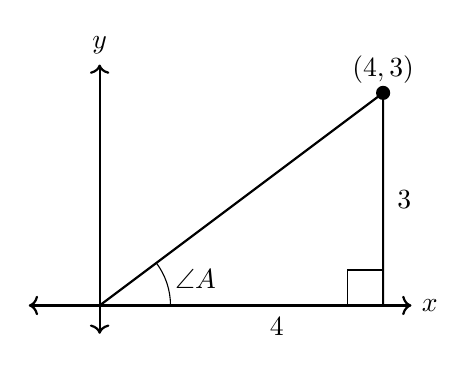
\begin{tikzpicture}[scale=0.9]
        \draw [thick, <->] (-1,0) -- (4.4,0) node [right] {$x$};
        \draw [thick, <->] (0,-0.4)--(0,3.4) node [above] {$y$};  
        \draw [thick] (0,0)--(4,0)--(4,3)--cycle;
        \draw (4,0) ++(-0.5,0)--+(0,0.5)--+(0.5,0.5);
        \node at (2.5,-0.3){4};
        %\node at (2,2.2){5};
        \node at (4.3,1.5){3};
        \fill (4,3) circle[radius=0.1] node[above] {$(4,3)$};
        \draw (1,0) arc (0:37:1)node[pos=0.6, right] {$\angle A$};
      \end{tikzpicture}
    \end{flushright}
  \end{columns}
\end{frame}

\begin{frame}{Standard notation for trigonometric functions}
  Right triangle $\triangle ABC$ with side lengths $a$, $b$, $c$. $m\angle A = \theta$
  \begin{center}
  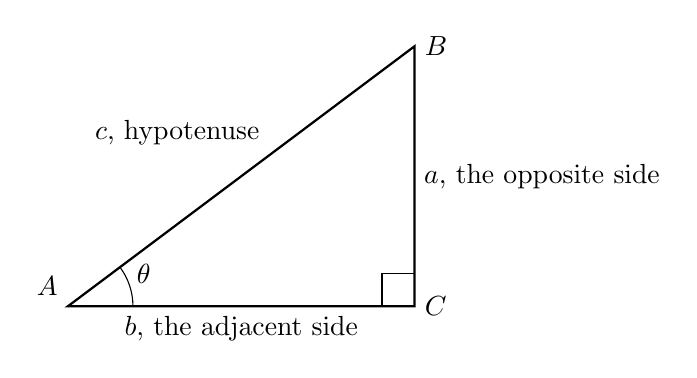
\begin{tikzpicture}[scale=0.55]
    \draw [thick](0,0)node[above left]{$A$}--
        (8,0)node[right]{$C$}--
        (8,6)node[right]{$B$}--cycle;
    \node at (1.75,0.75){$\theta$};
    \draw (1.5,0) arc (0:37:1.5);
    \draw (8,0) ++(-0.75,0)--+(0,0.75)--+(0.75,0.75);
    \node at (4,0) [below]{$b$, the adjacent side};
    \node at (8,3) [right]{$a$, the opposite side};
    \node at (0.4,4) [right]{$c$, hypotenuse};
  \end{tikzpicture}
  \end{center}
  \begin{description}
    \item[Opposite] The side across from the angle
    \item[Adjacent] The side next to the angle
    \item[Theta] A Greek letter used to represent the angle measure
    \item[tangent] The ratio of the opposite side to the adjacent side
  \end{description}
\end{frame}

\begin{frame}{Find the height of a triangle with base $b=10$ and angle 60 degrees}
  \begin{columns}
    \column{0.5\textwidth}
    \begin{center}
      $\displaystyle \tan(\theta)=\frac{opposite}{adjacent}$
      \end{center}
      Substitute the given values and use your calculator for $\tan(60^\circ)$
      \onslide<2>{\textcolor{red}{    
        \begin{center}
        $\displaystyle \tan(60^\circ)=\frac{a}{10} \approx 1.732$\\[0.5cm]
        $\displaystyle a=10\times 1.732 \approx 17.32$
        \end{center}}}
    \column{0.5\textwidth}
    \begin{flushright}
      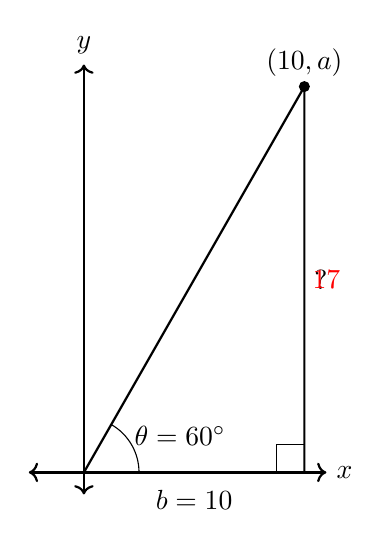
\begin{tikzpicture}[scale=0.7]
        \draw [thick, <->] (-1,0) -- (4.4,0) node [right] {$x$};
        \draw [thick, <->] (0,-0.4)--(0,7.4) node [above] {$y$};  
        \draw [thick] (0,0)--(4,0)--(4,7)--cycle;
        \draw (4,0) ++(-0.5,0)--+(0,0.5)--+(0.5,0.5);
        \node at (2,-0.5){$b=10$};
        \onslide<1>{\node at (4.3,3.5){?};}
        \onslide<2>{\node at (4.4,3.5){\textcolor{red}{17}};}
        \fill (4,7) circle[radius=0.1] node[above] {$(10,a)$};
        \draw (1,0) arc (0:60:1)node[pos=0.7, right] {$\theta = 60^\circ$};
      \end{tikzpicture}
    \end{flushright}
  \end{columns}
\end{frame}

\section{10.2 Inverse tangent function \hfill 18 April \,}
\begin{frame}{Learning Target: I can find an angle measure using inverse tangent.}
  {CCSS.HSG.SRT.C.8 Use trig ratios and the Pythagorean Theorem to solve problems \hfill \alert{10.2 Tuesday 18 April}}
  \begin{columns}
    \column{0.6\textwidth}
    Do Now: Given right $\triangle$ shown, find its height $b$ to the \emph{nearest tenth}. \\[0.5cm]
    Lesson: The inverse tangent function, $\tan^{-1}$ \\[0.5cm]
    Homework: Complete the classwork practice, Deltamath problem set
    \column{0.4\textwidth}
    \begin{flushright}
      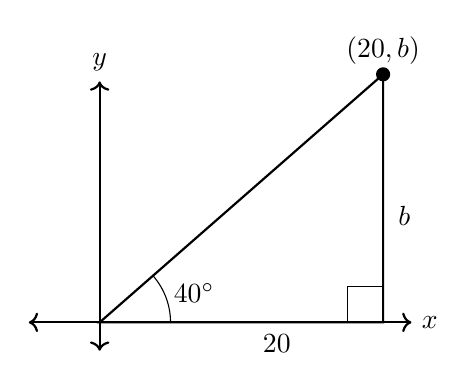
\begin{tikzpicture}[scale=0.9]
        \draw [thick, <->] (-1,0) -- (4.4,0) node [right] {$x$};
        \draw [thick, <->] (0,-0.4)--(0,3.4) node [above] {$y$};  
        \draw [thick] (0,0)--(4,0)--(4,3.5)--cycle;
        \draw (4,0) ++(-0.5,0)--+(0,0.5)--+(0.5,0.5);
        \node at (2.5,-0.3){20};
        \node at (4.3,1.5){$b$};
        \fill (4,3.5) circle[radius=0.1] node[above] {$(20,b)$};
        \draw (1,0) arc (0:41:1)node[pos=0.6, right] {$40^\circ$};
      \end{tikzpicture}
    \end{flushright}
  \end{columns}
\end{frame}

\section{10.3 Algebra practice \hfill 24 April \,}
\begin{frame}{Learning Target: I can model and solve with trigonometry algebra.}
  {CCSS.HSG.SRT.C.8 Use trig ratios and the Pythagorean Theorem to solve problems \hfill \alert{10.3 Monday 24 April}}
  \begin{columns}
    \column{0.6\textwidth}
    Do Now: Given right $\triangle$ with leg lengths 12.5 and 17.5. Find the angle measure $x$ to the \emph{nearest degree}. \\[0.5cm]
    Lesson: Practice modeling with tangent function and solving the algebra \\
      \alert{Calculator check} (it should be on your desk) \\[0.5cm]
    Homework: Complete the classwork practice, Deltamath problem set
    \column{0.4\textwidth}
    \begin{flushright}
      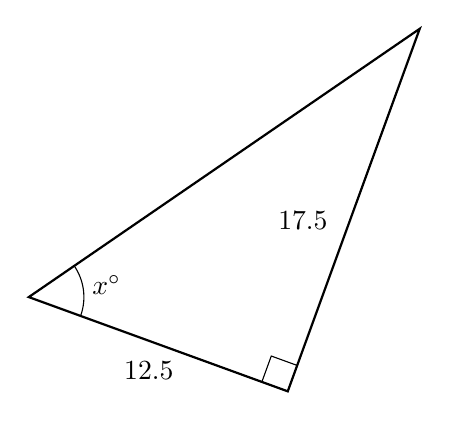
\begin{tikzpicture}[scale=0.7, rotate=-20] 
        \draw [thick] (0,0)--(5,0)--(5,7)--cycle;
        \draw (5,0) ++(-0.5,0)--+(0,0.5)--+(0.5,0.5);
        \node at (2.5,-0.5){12.5};
        \node at (4.2,3){17.5};
        \draw (1,0) arc (0:55:1)node[pos=0.6, right]{$x^\circ$};
      \end{tikzpicture}
    \end{flushright}
  \end{columns}
\end{frame}

\begin{frame}{Find the base of a triangle with height $h=10$ and angle 55 degrees}
  \begin{columns}
    \column{0.5\textwidth}
    \begin{center}
      $\displaystyle \tan(\theta)=\frac{opposite}{adjacent}$
      \end{center}
      Substitute the given values and use your calculator for $\tan(55^\circ)$
      \onslide<2>{\textcolor{red}{    
        \begin{center}
        $\displaystyle \tan(55^\circ)=\frac{10}{x}$\\[0.5cm]
        $\displaystyle x (1.428\ldots) = 10$\\[0.5cm]
        $\displaystyle x = \frac{10}{1.428\ldots} \approx 7.00 \ldots$
        \end{center}}}
    \column{0.5\textwidth}
    \begin{flushright}
      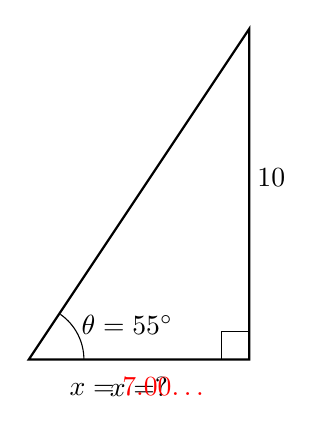
\begin{tikzpicture}[scale=0.7] 
        \draw [thick] (0,0)--(4,0)--(4,6)--cycle;
        \draw (4,0) ++(-0.5,0)--+(0,0.5)--+(0.5,0.5);
        \node at (4.4,3.3){10};
        \onslide<1>{\node at (2,-0.5){$x=$?};}
        \onslide<2>{\node at (2,-0.5){$x= \;$\textcolor{red}{7.00\ldots}};}
        \draw (1,0) arc (0:55:1)node[pos=0.7, right] {$\theta = 55^\circ$};
      \end{tikzpicture}
    \end{flushright}
  \end{columns}
\end{frame}


\section{10.4 Applications \hfill 25 April \,}
\begin{frame}{Learning Target: I can solve real world problems with trigonometry.}
  {CCSS.HSG.SRT.C.8 Use trig ratios and the Pythagorean Theorem to solve problems \hfill \alert{10.4 Tuesday 25 April}}
  \begin{columns}
    \column{0.5\textwidth}
    Do Now: Given right $\triangle$ shown, find its height $h$ to the \emph{nearest tenth}. \\[0.5cm]
    Lesson: Applying trigonometry to real world situations \\[0.5cm]
    Homework: Complete the classwork, Deltamath problem set \\
    \alert{Test Tuesday}
    \column{0.5\textwidth}
    \begin{flushright}
      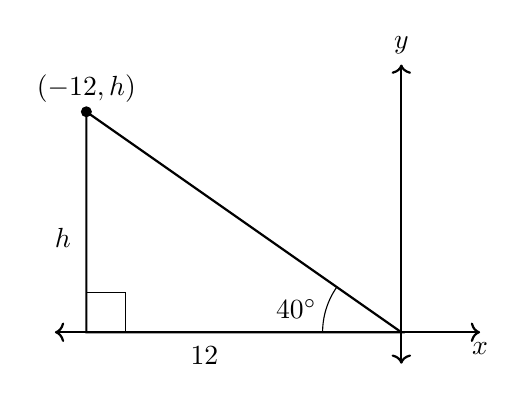
\begin{tikzpicture}[scale=1]
        \draw [thick, <->] (-4.4,0) -- (1,0) node [below] {$x$};
        \draw [thick, <->] (0,-0.4)--(0,3.4) node [above] {$y$};  
        \draw [thick] (0,0)--(-4,0)--(-4,2.8)--cycle;
        \draw (-4,0) ++(0.5,0)--+(0,0.5)--+(-0.5,0.5);
        \node at (-2.5,-0.3){12};
        \node at (-4.3,1.2){$h$};
        \fill (-4,2.8) circle[radius=0.07] node[above] {$(-12,h)$};
        \draw (-1,0) arc (180:145:1)node[pos=0.5,left] {$40^\circ$};
      \end{tikzpicture}
    \end{flushright}
  \end{columns}
\end{frame}

\begin{frame}{Applications to real world situations}
  For example: heights of trees, wires to a pole, lighthouses, buildings, airplanes...
  \begin{center}
  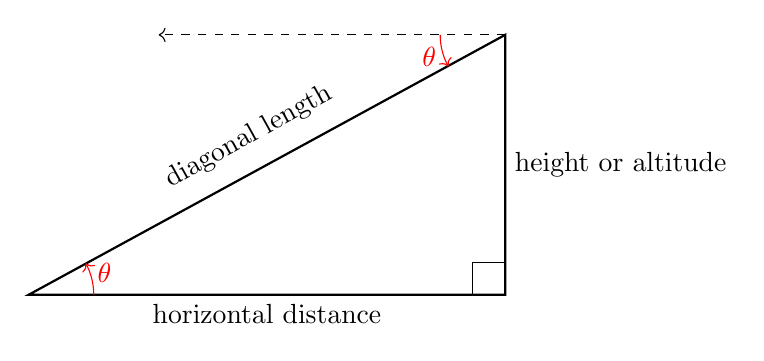
\begin{tikzpicture}[scale=0.55]
    \draw [thick](-3,0)--
        (8,0)--
        (8,6)--cycle;
    \draw [dashed, ->] (8,6)--(0,6);
    \node at (-1.25,0.5)[red]{$\theta$};
    \node at (6.25,5.5)[red]{$\theta$};
    \draw [->, red] (-1.5,0) arc (0:29:1.5);
    \draw [->, red] (6.5,6) arc (180:180+29:1.5);
    \draw (8,0) ++(-0.75,0)--+(0,0.75)--+(0.75,0.75);
    \node at (2.5,0) [below]{horizontal distance};
    \node at (8,3) [right]{height or altitude};
    \node at (0,2.5) [right, rotate=29]{diagonal length};
  \end{tikzpicture}
  \end{center}
  \begin{description}
    \item[Angle of elevation] The upward angle from the horizontal to line of sight
    \item[Angle of declination] The downward angle from the horizon to the object on the ground
    \item[Equal angles] The two alternate interior angles are congruent.
  \end{description}
\end{frame}

%10.5 was test review, out of order
\section{10.6 Applications \hfill 28 April \,}
\begin{frame}{Learning Target: I can solve real world problems with trigonometry.}
  {CCSS.HSG.SRT.C.8 Use trig ratios and the Pythagorean Theorem to solve problems \hfill \alert{10.6 Friday 28 April}}
  \begin{columns}
    \column{0.7\textwidth}
    Do Now: ``Solve'' the $\triangle$ shown. i.e. calculate the two angle measures and the length of the hypotenuse. \\[0.5cm]
    Lesson: Applying trigonometry in a variety of contexts \\
    \alert{Deltamath exit quiz} (10 minutes) \\[0.5cm]
    Homework: Complete the classwork practice \\
    \alert{Test Tuesday}
    \column{0.3\textwidth}
    \begin{flushright}
      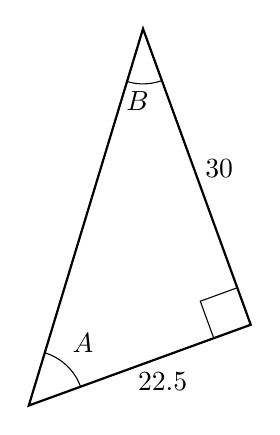
\begin{tikzpicture}[scale=1, rotate=20] 
        \draw [thick] (0,0)--(3,0)--(3,4)--cycle;
        \draw (3,0) ++(-0.5,0)--+(0,0.5)--+(0.5,0.5);
        \node at (1.7,-0.3){22.5};
        \node at (3.3,2){30};
        \draw (0.7,0) arc (0:53:0.7)node[pos=0.6, above right]{$A$};
        \draw (3,3.3) arc (-90:-127:0.7)node[pos=0.1, below left]{$B$};
      \end{tikzpicture}
    \end{flushright}
  \end{columns}
\end{frame}

\begin{frame}{Percentage grade of a road}
  Example: A road rising 30 feet for every 1000 feet of horizontal distance has a 3\% grade. \\[0.5cm]
  \begin{center}
  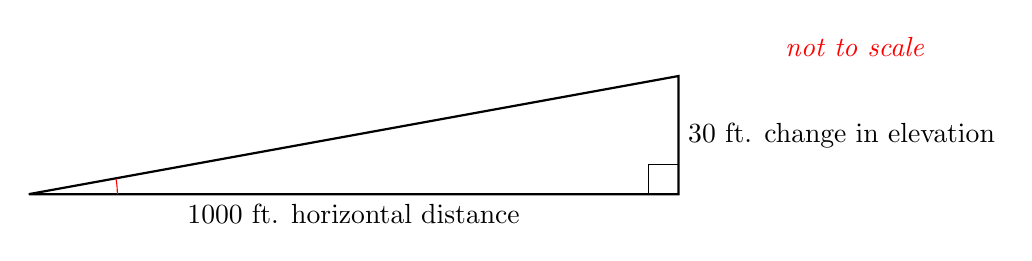
\begin{tikzpicture}[scale=0.75]
    \draw [thick](-3,0)--
        (8,0)--
        (8,2)--cycle;
    \node at (11,2.5)[red]{\emph{not to scale}};
    \draw [-, red] (-1.5,0) arc (0:10:1.5);
    \draw (8,0) ++(-0.5,0)--+(0,0.5)--+(0.5,0.5);
    \node at (2.5,0) [below]{1000 ft. horizontal distance};
    \node at (8,1) [right]{30 ft. change in elevation};
  \end{tikzpicture}
  \end{center}
  \begin{description}
    \item[Grade] The ratio of the vertical change to the horizontal change (percent)
    \item[Elevation] How high something is above sea level
    \item[Altitude] The height of an object above the ground
    \item[not to scale] proportions are not accurate
  \end{description}
\end{frame}

\section{10.7 Quiz: tangent function \hfill 2 May \,}
\begin{frame}{Learning Target: I can use the tangent function and solve problems with trigonometry.}
  {CCSS.HSG.SRT.C.8 Use trig ratios and the Pythagorean Theorem to solve problems \hfill \alert{10.7 Tuesday 2 May}}

    Do Now: Turn in Unit 10 problem sets, stapled in reverse order \\[0.5cm]
    Test: Use your notebook and calculator (no computers) \\[0.5cm]
    \emph{Do not share calculators} \\[0.5cm]
    Early finishers: Deltamath Regents review
\end{frame}

\section{10.8 Sine and cosine functions \hfill 3 May \,}
\begin{frame}{Learning Target: I can use the sine and cosine functions}
  {CCSS.HSG.SRT.C.8 Use trig ratios and the Pythagorean Theorem to solve problems \hfill \alert{10.8 Wednesday 3 May}}
  \begin{columns}
    \column{0.7\textwidth}
    Do Now: Calculate the length of the base $x$ and the two angle measures. \\[0.5cm]
    Lesson: Using $\sin \theta$ and $\cos \theta$ \\[0.5cm]
    Homework: Complete the classwork practice, Deltamath \\
    \column{0.3\textwidth}
    \begin{flushright}
      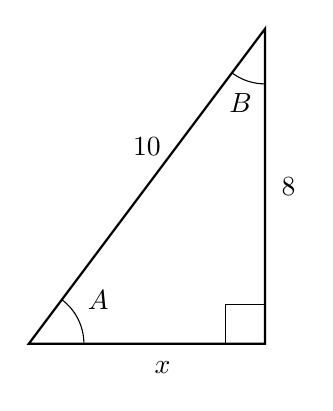
\begin{tikzpicture}[scale=1] 
        \draw [thick] (0,0)--(3,0)--(3,4)--cycle;
        \draw (3,0) ++(-0.5,0)--+(0,0.5)--+(0.5,0.5);
        \node at (1.5,2.5){10};
        \node at (1.7,-0.3){$x$};
        \node at (3.3,2){8};
        \draw (0.7,0) arc (0:53:0.7)node[pos=0.5, above right]{$A$};
        \draw (3,3.3) arc (-90:-127:0.7)node[pos=0.1, below left]{$B$};
      \end{tikzpicture}
    \end{flushright}
  \end{columns}
\end{frame}

\begin{frame}{Sine and cosine trigonometric functions}
  Right triangle $\triangle ABC$ with side lengths $a$, $b$, $c$. $m\angle A = \theta$
  \begin{center}
  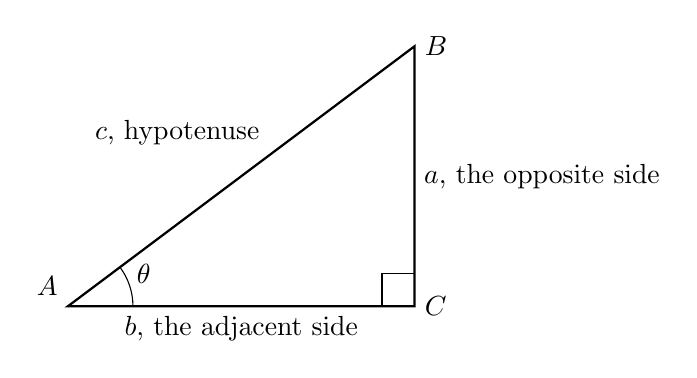
\begin{tikzpicture}[scale=0.55]
    \draw [thick](0,0)node[above left]{$A$}--
        (8,0)node[right]{$C$}--
        (8,6)node[right]{$B$}--cycle;
    \node at (1.75,0.75){$\theta$};
    \draw (1.5,0) arc (0:37:1.5);
    \draw (8,0) ++(-0.75,0)--+(0,0.75)--+(0.75,0.75);
    \node at (4,0) [below]{$b$, the adjacent side};
    \node at (8,3) [right]{$a$, the opposite side};
    \node at (0.4,4) [right]{$c$, hypotenuse};
  \end{tikzpicture}
  \end{center}
  \begin{description}
    \item[tangent] The ratio of the opposite side to the adjacent side
    \item[sine] The ratio of the opposite side to the hypotenuse
    \item[cosine] The ratio of the adjacent side to the hypotenuse
    \item[SOH CAH TOA] \emph{mnemonic device}
  \end{description}
\end{frame}

\begin{frame}{Find the legs of a triangle with hypotenuse $c=20$ and angle 60 degrees}
  \begin{columns}
    \column{0.5\textwidth}
    \begin{center}
      $\displaystyle \sin(\theta)=\frac{opposite}{hypotenuse}=\frac{a}{c}$ \\[0.3cm]
      $\displaystyle \cos(\theta)=\frac{adjacent}{hypotenuse}=\frac{b}{c}$
      \end{center}
      Substitute the given values and solve
      \onslide<2>{\textcolor{red}{    
        \begin{center}
        $\displaystyle \sin(60^\circ)=\frac{a}{20} = 0.866 \ldots$\\[0.3cm]
        $\displaystyle a=20\times 0.866 \ldots \approx 17.3$ \\[0.5cm]
        $\displaystyle \cos(60^\circ)=\frac{b}{20} = 0.5$\\[0.3cm]
        $\displaystyle b=20\times 0.5 = 10$
        \end{center}}}
    \column{0.5\textwidth}
    \begin{flushright}
      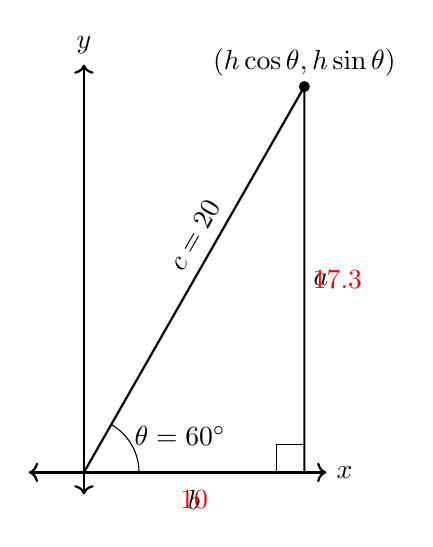
\begin{tikzpicture}[scale=0.7]
        \draw [thick, <->] (-1,0) -- (4.4,0) node [right] {$x$};
        \draw [thick, <->] (0,-0.4)--(0,7.4) node [above] {$y$};  
        \draw [thick] (0,0)--(4,0)--(4,7)--cycle;
        \draw (4,0) ++(-0.5,0)--+(0,0.5)--+(0.5,0.5);
        \node[rotate=60] at (2,4.3){$c=20$};
        \onslide<1>{\node at (4.3,3.5){$a$};}
        \onslide<2>{\node at (4.6,3.5){\textcolor{red}{17.3}};}
        \onslide<1>{\node at (2,-0.5){$b$};}
        \onslide<2>{\node at (2,-0.5){\textcolor{red}{10}};}
        \fill (4,7) circle[radius=0.1] node[above] {$(h\cos \theta,h\sin \theta)$};
        \draw (1,0) arc (0:60:1)node[pos=0.7, right] {$\theta = 60^\circ$};
      \end{tikzpicture}
    \end{flushright}
  \end{columns}
\end{frame}

\section{10.9 Inverse trig functions \hfill 4 May \,}
\begin{frame}{Learning Target: I can use the sine and cosine inverse}
  {CCSS.HSG.SRT.C.8 Use trig ratios and the Pythagorean Theorem to solve problems \hfill \alert{10.9 Thursday 4 May}}
  \begin{columns}
    \column{0.7\textwidth}
    Do Now: Calculate the length of the base $x$ and the two angle measures. \\[0.5cm]
    Lesson: Using $\sin \theta$ and $\cos \theta$ \\[0.5cm]
    Homework: Complete the classwork practice, Deltamath \\
    \column{0.3\textwidth}
    \begin{flushright}
      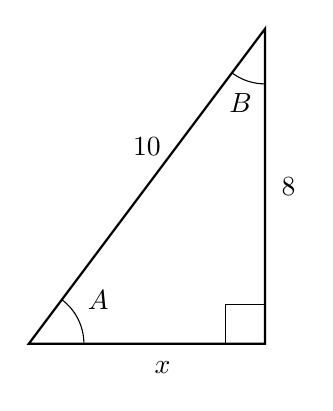
\begin{tikzpicture}[scale=1] 
        \draw [thick] (0,0)--(3,0)--(3,4)--cycle;
        \draw (3,0) ++(-0.5,0)--+(0,0.5)--+(0.5,0.5);
        \node at (1.5,2.5){10};
        \node at (1.7,-0.3){$x$};
        \node at (3.3,2){8};
        \draw (0.7,0) arc (0:53:0.7)node[pos=0.5, above right]{$A$};
        \draw (3,3.3) arc (-90:-127:0.7)node[pos=0.1, below left]{$B$};
      \end{tikzpicture}
    \end{flushright}
  \end{columns}
\end{frame}

\section{10.10 Special triangles \hfill 5 May \,}
\begin{frame}{Learning Target: I can calculate exact values using special triangles}
  {CCSS.HSG.SRT.C.8 Use trig ratios and the Pythagorean Theorem to solve problems \hfill \alert{10.10 Friday 5 May}}
  \begin{columns}
    \column{0.7\textwidth}
    Do Now: Calculate the triangle's height $h$ and the two angle measures. \\[0.5cm]
    Lesson: $30-60-90$ and $45-45-90$ triangles. \\[0.5cm]
    Homework: Complete the classwork practice, Deltamath \\
    \column{0.3\textwidth}
    \begin{flushright}
      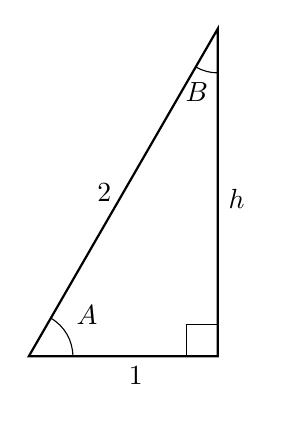
\begin{tikzpicture}[scale=0.8] 
        \draw [thick] (0,0)--(3,0)--(3,5.2)--cycle;
        \draw (3,0) ++(-0.5,0)--+(0,0.5)--+(0.5,0.5);
        \node at (1.2,2.6){2};
        \node at (1.7,-0.3){1};
        \node at (3.3,2.5){$h$};
        \draw (0.7,0) arc (0:60:0.7)node[pos=0.5, above right]{$A$};
        \draw (3,4.5) arc (-90:-120:0.7)node[pos=0.0, below left]{$B$};
      \end{tikzpicture}
    \end{flushright}
  \end{columns}
\end{frame}

\end{document}
